%*********************第二章******************
\chapter{基于大规模多核CPU系统的心脏组织的3D精细模拟}
\label{ICA3PP}

\section{引言}
细胞内钙离子处理功能异常被认为是几个心脏病理(比如心脏衰竭\upcite{marks2013calcium,kubalova2005abnormal},心脏肥大\upcite{berridge2006remodelling},心肌病\upcite{pieske1995alterations}以及肌浆网内钙离子释放处理紊乱\upcite{liu2006arrhythmogenesis,priori2011inherited})的极有可能的诱因。上述心脏疾病中的大多都是源于亚细胞内微米级和纳米级上钙离子释放处理功能不正常造成的,表现为由t-型管畸形\upcite{louch2004reduced,louch2006t,van2011disrupted}和单兰尼碱受体功能紊乱\upcite{liu2006arrhythmogenesis,jiang2005enhanced}造成心脏的病理。

在过去的几年里,数值方法和计算技术的进步使得心脏细胞的电生理学和钙离子处理模型得到了快速发展,这些模型也开始考虑亚细胞中的随机钙离子释放过程\upcite{restrepo2008calsequestrin,gaur2011multiscale,nivala2012computational,williams2011dynamics}的离散特性。新一代的钙离子处理和动作电位模型在研究心律失常的机制和预防具有非常重要的价值,心律失常主要因为细胞内纳米级钙离子释放通道和dyadic单元功能的紊乱进而影响亚细胞级的膜电位的不正常而造成的,膜电位的异常通常表现为去极化延迟、过早地去极化\upcite{song2015calcium}以及心脏电交替变化\upcite{restrepo2008calsequestrin,nivala2012calcium,nivala2015t}。虽然这些发展能让我们从不同尺度的动作电位对心律失常进行理解,这些尺度可以从单通道到整个细胞,然而我们仍然面临很多挑战。

首先,心律失常发生在心脏组织级和器官级。从细胞这一层级的研究对心脏组织和器官的心律失常进行理解推断往往不是特别清楚,有时反而不利于进行研究。其次,从心脏组织这个层次进行研究已经被证明对计算有极大的需求。一个典型的人类心脏大概有$2 \times 10^9 $个细胞\upcite{adler1974cell},每个细胞内大概有$10^6$个RyRs和约$10^5$个L型通道,这些通道的功能就是对膜电位和细胞内各个单元里的钙离子浓度进行随机的作出响应\upcite{cheng1993calcium}。在心脏组织级这个层次的真实模拟不仅需要大量的并行计算节点,也需要复杂的算法设计,才能在合理的时间内对心脏的生理过程进行模拟。并且,到目前为止,还没有在心脏组织级这个层次采用精细的钙离子处理细胞模型对心律失常的机制进行研究。

本章主要介绍了在心脏组织中的电活动和钙离子处理的3D并行模拟器,所谓的并行模拟器就是对模拟过程在大规模的多核CPU系统中进行并行加速。本章首先会介绍关于心脏组织模拟的背景以及相关工作;然后将具体介绍本课题研究中所采用的数学模型,包括心脏组织级的数学模型和细胞内的数学模型;第三部分将介绍心脏组织模拟在多核CPU集群上的实现过程,包括节点内和节点间的并行实现以及单个细胞内的模拟过程的实现;最后是对心脏组织内各个单元的电位变化以及钙离子浓度变化的模拟,实验结果表明,本课题提出的精细的细胞模型能够很好地对心脏组织内的活动进行模拟。

%\section{相关研究}
%\subsection{心脏组织模拟的数学模型}
%\subsection{心脏组织模拟的并行实现}


\section{心脏组织3D模拟的数学模型和数值方法}

\subsection{组织级的数学模型}
心脏组织级模拟是通过公式 \ref{tissuevoltage}来描述的,该模型也叫单域模型。

\begin{equation}
\frac{\partial V_{m}}{\partial t}=\frac{-I_\mathrm{ion}}{C_{m}} + D_{x}\frac{\partial^{2}V_{m}}{\partial x^{2}}+D_{y}\frac{\partial^{2}V_{m}}{\partial  y^{2}}+D_{z}\frac{\partial^{2}V_{m}}{\partial z^{2}},
\label{tissuevoltage}
\end{equation}

公式\ref{tissuevoltage}中$V_{m}$为膜电位,$I_\mathrm{ion}$为组织模拟中主要涉及的离子流动产生的电流,$C_{m}=1\mu F cm^{-2}$ 是细胞内膜间电容,$D_{x}=D_y=D_z=0.2 $ $mm^{2}/ms$是电压在三维空间上各个坐标方向的扩散系数。心脏3D组织级模型中,3D组织是由众多心脏细胞构成的,而心脏细胞的模型是采用\ref{cellmodel}中描述的模型。

有限差分法结合算子分裂方法\upcite{qu1999advanced}被用来对公式\ref{tissuevoltage}进行离散化。这意味着扩散项与离子的电流项$I_\mathrm{ion}$分别进行处理。电流项需要通过求解每个细胞的精细模型方程而得到。细胞内的精细模型将在\ref{cellmodel}进行介绍。

\subsection{细胞级的数学模型}
\label{cellmodel}

 本课题借鉴了文献\upcite{gaur2011multiscale}在心肌细胞内采用随机钙离子处理的多尺度模型。为了模拟人类心脏组织细胞,本课题使用O'Hara-Rudy (ORd)的心脏电位公式\upcite{o2011simulation}替换了文献\upcite{gaur2011multiscale}中的电生理电流公式,ORd模型是针对健康人类的心脏细胞的模拟,而文献\upcite{gaur2011multiscale}中描述的是豚鼠的模型。
 
 \begin{figure}[ht]
\center
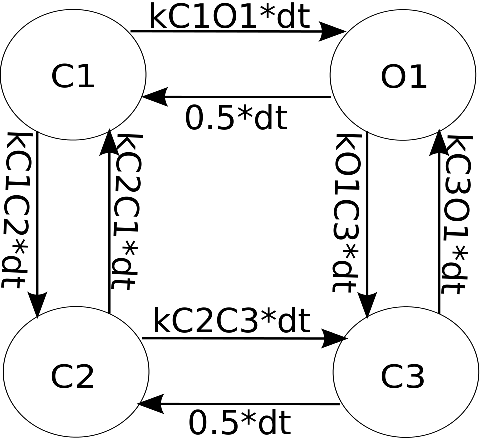
\includegraphics[scale=0.5]{figs/state.pdf}
\caption{The eight possible transitions between four states of a RyR, where the labels on the arrows indicate the
probabilities of the transitions.}
\label{ryrstates}
\end{figure}

在每个细胞里,有约$10000$个钙离子释放单元也叫dyads,这些钙离子释放单元按照$100\times 10\times 10$的三维网格进行排列。每个dyad包含五个不同的小单元,钙离子会在这些小单元里停留,详细的公式和参数可以参考文献\upcite{gaur2011multiscale}。每个dyad空间里,包含15个L-型钙离子通道和$100$个RyRs,它们是随机地活动的。在任何时刻,每个RyR会处于四个状态中的一个,这四个状态用C1、~C2、~C3以及~O1表示。图\ref{ryrstates}中给出了各个状态间可能的转换关系,以及状态间转换的概率,图\ref{ryrstates}状态转换的概率参数是与每个RyR内的钙离子浓度相关的,除了其中从~O1到~C1以及从~C3到~C2的转换概率为常数。处于打开状态(即处于~O1状态)的RyR的个数直接影响到钙离子的流量,进而影响每个细胞内的电压。

dyad中的钙离子浓度可以通过公式\ref{eq:1}至公式\ref{eq:10}来求解。

{
\allowdisplaybreaks
 \begin{eqnarray}
  ca_{\mathrm{ds}}& = & (J_{\mathrm{rel}} + J_{\mathrm{lca}} + ca_{\mathrm{ss}} / \tau_{\mathrm{efflux}})\times \tau_{\mathrm{efflux}}\label{eq:1}\\
  \frac{d\, ca_{\mathrm{ss}}}{dt}& = & \overline{B_{\mathrm{ss}}}\left(  J_{\mathrm{NCX}} + J_{\mathrm{diff\_myo\_ss}} + J_{\mathrm{diff\_ds\_ss}}\right) \label{eq:2}\\
  \frac{d\,ca_{\mathrm{JSR}}}{dt}& = & \overline{B_{\mathrm{JSR}}}\left(J_{\mathrm{rel}} + J_{\mathrm{diff\_NSR\_JSR}}\right) \label{eq:3}\\
  \frac{d\,ca_{\mathrm{NSR}}}{dt}& = & J_{\mathrm{up}} - J_{\mathrm{leak}} - J_{\mathrm{diff\_NSR\_JSR}}  \label{eq:4}\\ 
  \frac{d\,ca_{\mathrm{myo}}}{dt}& = & \overline{B_{\mathrm{myo}}}\left(J_{\mathrm{cab}} + J_{\mathrm{pca}} + J_{\mathrm{NCX}} - J_{\mathrm{up}} + J_{\mathrm{leak}} - J_{\mathrm{diff\_myo\_ss}}\right) \label{eq:5}\\
  Ca_{\mathrm{ds}}& = & (J_{\mathrm{rel}} + J_{\mathrm{lca}} + Ca_{\mathrm{ss}} / \tau_{\mathrm{efflux}})\times \tau_{\mathrm{efflux}}\label{eq:6}\\  
  \frac{\partial Ca_{\mathrm{ss}}}{\partial t}& = & \overline{B_{\mathrm{ss}}} \left(J_{\mathrm{NCX}} + J_{\mathrm{diff\_myo\_ss}} + J_{\mathrm{diff\_ds\_ss}}
+ D_{Ca}\nabla^2Ca_{\mathrm{ss}}\right) \label{eq:7}\\
  \frac{d\,Ca_{\mathrm{JSR}}}{dt}& = & \overline{B_{\mathrm{JSR}}}\left(J_{\mathrm{rel}} + J_{\mathrm{diff\_NSR\_JSR}}\right) \label{eq:8}\\
  \frac{\partial Ca_{\mathrm{NSR}}}{\partial t}& = & J_{\mathrm{up}} - J_{\mathrm{leak}} - J_{\mathrm{diff\_NSR\_JSR}}  +  D_{\mathrm{SR}}\nabla^2 Ca_{\mathrm{NSR}}\label{eq:9}\\					
  \frac{\partial Ca_{\mathrm{myo}}}{\partial t}& = &
                                                     \overline{B_\mathrm{myo}}\left(J_\mathrm{cab} + J_\mathrm{pca} + J_\mathrm{NCX} - J_\mathrm{up} + J_\mathrm{leak} - J_\mathrm{diff\_myo\_ss}\right.\nonumber\\
&&+ \left. D_{Ca}\nabla^2Ca_{\mathrm{myo}}\right)
\label{eq:10}
  \end{eqnarray}
}
%
%\noindent

公式中,$J_{\mathrm{rel}}$是从RyRs到dyad单元间的钙离子流通量,$J_{\mathrm{lca}}$是从L-型钙离子通道到dyad间的钙离子流通量,$\tau_{\mathrm{efflux}}$是dyad空间和膜下空间之间的扩散系数,$J_{\mathrm{NCX}}$是钠离子和钙离子交换在膜下空间产生的电流通量,$J_{\mathrm{diff\_myo\_ss}}$是肌质与膜下空间之间的扩撒流通量,$J_{\mathrm{diff\_ds\_ss}}$是dyad与膜下空间之间的扩撒流通量。$J_{\mathrm{diff\_NSR\_JSR}}$是NSR和JSR间的扩撒流通量,SR泵可以将钙离子从NSR抽到SR中,产生的流通量用$J_{\mathrm{leak}}$来表示。$J_{\mathrm{pca}}$是流过胞质膜的钙离子流通量,膜下空间会被SR和SL瞬间缓冲,瞬间缓冲系数是通过$\overline{B_{\mathrm{ss}}}$来表示的。$\overline{B_{\mathrm{JSR}}}$是CSQN到JSR间的瞬间缓冲系数,$\overline{B_{\mathrm{myo}}}$是从CMDN和TRPN到胞质膜的瞬间缓冲系数。更加详细的关于各个参数和变量的信息可以参考文献\upcite{gaur2011multiscale}。

\subsection{数值策略}
本课题采用随机的方法对L-型钙离子通道和RyRs进行随机模拟,详细的介绍将在\ref{cellImp}中介绍。显式时间积分法被用来求解所有的微分方程(\ref{tissuevoltage})-(\ref{eq:10})。涉及的扩撒项采用中心有限差分的方法进行离散化。而对于单域方程(\ref{tissuevoltage}),使用的是算子分裂方法\upcite{qu1999advanced}。这意味着扩撒项与离子产生的电流项$I_\mathrm{ion}$是分开处理的,后者是通过求解Ord模型中的所有常微分方程得到所有的离子电流,并将所有的离子电流累加起来而得到。

所有的计算流程是发生在一个时间循环内,循环中是每个时间步需要完成的工作,具体包括对所有细胞内的模拟,然后是根据公式\ref{tissuevoltage}对细胞间电压扩撒过程进行计算。每个细胞内的计算包括对所有的dyads进行计算,然后对dyad间的扩撒过程进行计算。具体过程如表\ref{overview}中的伪代码所示,对其中的计算进行高效实现变得非常重要。

\begin{table}
\caption{3D组织模拟计算的伪代码实现}
\label{overview}
\begin{lstlisting}[language=C++, basicstyle=\ttfamily\footnotesize]
Global initialization
  for (int t = 0; t < time steps; t++) {	
    for (int k = 1; k <= cells; k++) {
      Cell computation
      for (int j = 1; j <= dyads; j++) {
        L-type probability calculation
        L-type opening	
        RyR probability calculation
        RyR opening
        Ca concentration computation }
      Dyad diffusion }
    Cell difusion }
\end{lstlisting}
\end{table}

\section{基于多核CPU系统的心脏组织3D模拟的实现}

 \subsection{多级并行}

在介绍大规模心脏组织模拟的实现之前,先介绍实现所面向的目标平台以及相应的编程模型。本课题面向的是多核CPU集群系统,集群中节点间通过以太网或者光纤高速互联,节点间通信可以通过MPI实现,在单节点内也可以创建多个MPI进程进行通信。本课题采用了MPI进行编程,每个MPI进程控制一个计算节点,节点间通过MPI进程进行通信,这种编程方式可移植性好,方便程序员显式控制通信。对于单节点内部来说,每个节点都是由多核CPU构成的,为了充分利用多核CPU的计算资源,本课题采用OpenMP的编程方法,为每一个CPU核分配相应的任务。对于其中的CPU核来说,由于CPU支持向量化执行,因此,还可以进一步利用硬件的并行计算资源。

基于现有的目标平台以及编程模型,本课题采用了一种多级并行策略对大规模心脏组织的模拟进行加速。首先是将3D心脏组织网格划分成很多子网格,每一个网格中的所有细胞的模拟分配给一个计算节点完成,而对于网格中的所有细胞的模拟,由于各个细胞的模拟是相互独立的过程,因此可以采用OpenMP对细胞的模拟并行执行。MPI通信只发生在组织层,因为在计算扩散项\ref{tissuevoltage}时,当前细胞的电压与相邻的细胞的电压有关,这就会涉及到MPI通信了。然而主要的计算还是发生在细胞内, \label{cellImp}将重点介绍单个细胞内的计算的实现。
 
 \subsection{单个细胞内的数值计算实现}
 \label{cellImp}
 在细胞内的所有计算中,最耗时的计算部分是关于钙离子处理的那部分。因此,本节重点关注这部分计算,暂且将这部分计算命名为{\tt computeCalciumInDyad},表\ref{cellfunction}中展示的是该部分计算的伪代码。
 
 \begin{table}
\caption{The function that implements calcium handling per cell.}
\label{cellfunction}
\begin{lstlisting}[language=C++, basicstyle=\ttfamily\footnotesize]
void computeCalciumInDyad()
    {
        generateRandData();
        for(int i=0;i<Ndyads;i++) {
            computateLocalLtypeCurrent();
            computeLocalSRCaRelease();
            computeLocalCaConcentration();
        }
        computeCaConcentrationDiffusion();
    }
\end{lstlisting}
\end{table}

 函数{\tt  computeCalciumInDyad}的计算复杂性直接与dyads的数目成正比,还可以看到函数{\tt  computeCalciumInDyad}中调用了五个函数,其中函数{\tt generateRandData}负责产生大量的随机数,每个时间迭代步中都需要重新产生新的随机数,这些随机数在细胞内L-通道的开和关的模拟中被使用到。函数{\tt  computeCaConcentrationDiffusion}是用来计算细胞内dyad间钙离子扩散中的浓度变化。另外三个函数将在一个{\tt for}循环中调用,特别的,函数{\tt computeLocalSRCaRelease}中的主要部分是计算每个dyad内$100$个RyRs状态间的随机转换过程。在接下来的内容中,将展现三个对并行模拟器性能产生影响的编程和数值技术。
 
 \subsubsection{避免重复计算}
在每个dyad的计算中,都需要计算大量的变量,有些变量在不同的dyad内值是不一样的,因此,对于这些变量,每一个dyad发生的计算中都应该包含这些变量的计算。然而,对于有些变量,其值对于所有的dyad都是相同的,由于dyad数量最多可以达到$10000$,,如果在进入对dyad的{\tt for}循环之前,预先将这些在每一次时间迭代步内不会改变的变量的值计算出来,可以大大减少计算的次数。这需要从这些复杂的公式中找出循环常量,根据实验的性能提升可以发现这些努力是值得的。

\subsubsection{细胞内的dyad间扩散的向量化}
细胞内的$10000$ 个dyads形成一个$100\times10\times10$的网格,钙离子由于浓度不同会在这些dyad间扩散。表\ref{diffusion}中的伪代码是这种3D扩散的计算实现过程,代码主要由三个{\tt for}循环构成,其中计算主要集中在最内的循环,最内的循环次数为$100$,因此可以考虑对该循环进一步优化。由于CPU核已经在细胞级采用OpenMP并行了,每个CPU核负责细胞内的计算,如果需要对细胞内的计算进一步并行,只能开发CPU核内的并行计算资源了。本课题采用的是Intel CPU,每个CPU核内具有256位的向量计算单元,所以对于64位双精度浮点计算来说,每个CPU一次可以处理4个双精度的浮点运算。由于dyad内的数据在$x$方向连续存储的,最内循环适合进行向量化。本课题通过添加编译指导语句,借助编译器对特定的循环进行向量化优化。理论上应该可以取得4倍的加速,但由于扩散中的计算是存储受限的计算,实际取得的性能提升将远低于理论上能取得的性能。

 \begin{table}
\caption{Pragma guided vectorization (in the $x$ direciton) of one of three diffusion computations between the dyads in function {\tt computeCaConcentrationDiffusion}.}
\label{diffusion}
\begin{lstlisting}[language=C++, basicstyle=\ttfamily\footnotesize]
for(z=1;z<Nz_diff-1;z++)
        for(y=1;y<Ny_diff-1;y++) {     
           int x,c,n,s,b,t;         
           x=0;
           c=x+y*Nx_diff+z*Nx_diff*Ny_diff;
           n=c-Nx_diff;            s=c+Nx_diff;
           b=c-Nx_diff*Ny_diff;    t=c+Nx_diff*Ny_diff; 
           
           U[c]=u[c]+fx*(2*u[c+1]-2*u[c])+fy*(u[n]+u[s]-2*u[c])
                    +fz*(u[b]+u[t]-2*u[c]);
           #pragma ivdep
           for(x=1;x<Nx_diff-1;x++) {
              ++c; ++n; ++s; ++b; ++t;
              U[c]=u[c]+fx*(u[c-1]+u[c+1]-2*u[c])+fy*(u[n]+u[s]-2*u[c])
                       +fz*(u[b]+u[t]-2*u[c]);              
           }
           U[c]=u[c]+fx*(2*u[c-1]-2*u[c])+fy*(u[n]+u[s]-2*u[c])
                                         +fz*(u[b]+u[t]-2*u[c]);
        }   \end{lstlisting}
\end{table}


\subsubsection{采用二项分布}
\label{binom}
%
前面的章节中已经介绍了每个dyad内包含$100$ RyRs,每个RyR在任何时刻会处于四种状态中的一种状态,在\ref{cellmodel}已经介绍了这四种状态,以及这四种状态间的转变关系,状态间的转变是按照一定的概率随机转变的。现在的目标是计算RyR中处于打开状态(O1)的数目,因为打开状态的RyR能够决定钙离子流量而影响细胞内电压,一种直接的方法是对每个RyR独立地进行模拟。这样每个dyad内需要消耗100个随机数对这100个RyRs的状态转变进行模拟。每个RyR根据当前状态以及相关的转变概率转变到另一个状态中,这种模拟的方法需要消耗大量的计算,一方面是因为需要消耗大量的随机数,随机数在每个时间步中都需要重新产生;另一方面,这种模拟实现中,代码含有大量的{\tt if}测试语句。

因此,如果能将dyad内的100个RyRs看作一个整体,直接计算出处于开放状态的RyR的数目,将有效降低计算量。因此,本课题将原本100次独立的随机试验替换为在一个二项分布中进行八次随机抽样的实验,对图\ref{ryrstates}中的每一次转变进行一次抽样试验。在二项分布中,$n$次试验中成功$k$次的概率为$p$,则$p$可以用公式\ref{eq:cumulative}计算。

\begin{equation}
F(k,n,p)=Pr({X}\leq{k})=\sum_{i=0}^{k}\binom{n}{i}p^i(1-p)^{n-i},
\label{eq:cumulative}
\end{equation}
式中$$\binom{n}{i}=\frac{n!}{i!(n-i)!}$$为二项系数。由于处于各个状态的RyRs的数目是从$0$ 到$100$间变化,可以预先计算好所有的二项系数,这也能显著提高计算性能。

使用服从$[0,1]$的均匀分布的随机数,对二项分布进行采样找出最小的$k$,使得$r \leq F(k,n,p)$。然而标准的二项分布实现对计算需求比较大,本课题采用了一个高效的实现,如表\ref{fig:binom}中代码所示。因为二项分布的系数预先已经计算出来了,只需要在每一轮试验中将$p/(1-p)$与基概率$(1-p)^n$相乘,并与二项系数相乘然后保存结果。

 \begin{table}
\caption{Implementation of Binomial Distribution Method. Function {\tt constant\_p\_binomial} simply finds $k$ by using the precomputed lookup table. In function {\tt binomial},
we first test if the computation can be skipped, using the threshold $p_t$ and the precomputed value $F(0,n,p_t)$. If this is not the case, the distribution function $F(k,n,p)$ is computed iteratively by subtracting from {\tt randValue} using the precomputed binomial coefficients.}
\label{fig:binom}
\begin{lstlisting}[language=C++, basicstyle=\ttfamily\footnotesize]
    int constant_p_binomial(n,randValue) {
        k=0;
        while(randValue>Table[n,k]) 
            k++;
        return k;
    }

    int binomial(n,p,randValue) {
        	if n = 0
		    return 0;
        if p < Threshold AND randValue < Precomp[n]
            return 0;
        k = 0;
        p_current =pow((1-p),n);
        p_step = p/(1-p);
        while(randValue > 0) {
            k++;
            randValue -= Binom[n,k]*p_current;
            p_current *= p_step;
        }
        return k;
    }  
           \end{lstlisting}
\end{table}

为了表示方便,用$x_1$,$x_2$,$x_3$,$x_4$这四个变量代表RyR处在四种状态的数目,并用$x_{ij}$表示RyR从状态$i$到状态$j$间的数目,$x_{ij}$是通过上述描述的方法通过对二项分布采用计算出来的。因此,在下一个时间步,处于各个状态的RyR数目可以用公式\ref{transitNumber}计算。

\begin{equation}
\label{transitNumber}
x_i = x_i - \sum_{j}x_{ij}+\sum_{j}x_{ji}.
\end{equation}

基于此,本课题根据细胞模型的特点增加了两个优化方法,在本课题中提出的细胞模型中,RyR中的状态中,从O1到C1和从C3到C2的转化概率为常数,即$p_c=0.5*dt$。因此,可以仿照预先计算二项系数的思路,也预先计算全部的累积概率函数$F(k,n,p_c)$。在这两种方法中,唯一的代价是需要存储$101*100/2=5050$个双精度浮点值,这增加了一些额外的存储开销。

另外,本课题还利用了细胞模型中另一个特性,就是RyR中大部分时间都是处于C2状态的,并且状态间的转变概率除了上述所说的两个为常数概率,其它转变概率在大部分时间都是接近0的。这意味着通过从二项分布中采样计算出的转变的RyR的数目也接近0。本课题通过设置一个小的概率阈值记为 $p_t$,并且对于所有的$0 \leq n \leq 100$,预先计算出$F(0,n,p_t)$ 。如果$p \leq p_t$,只要检查随机数$r$,看是否满足$r \leq F(0,n,p_t)$,如果满足,则$k=0$,代表没有发生状态转变,就可以不用计算二项分布了。当然,如果转变前处在某个状态的RyR数为0,那么发生状态转变的RyR数也为0,详细的代码参见表\ref{fig:binom}.

采用二项分布对RyR状态转变进行模拟的方法也在文献\upcite{restrepo2008calsequestrin}中被采用了,然而作者并没有去计算实际的二项分布,而是采用正态分布和泊松分布对其进行逼近,不过这会降低模拟的精度。
   
   
\section{实验结果与分析}
\subsection{实验设置}

本课题的测试系统是在Abel\upcite{abel}机器上,这是一个由奥斯陆大学管理维护的一个超级计算机系统。在Abel机器上的每个计算节点由Intel Xeon E5-2670处理器构成,共有16个物理计算核心,每个计算核心的频率为2.6GHz,由FDR Infiniband互联(56 Gbps)。本课题最多使用了128个计算节点(即2048个CPU核)进行数值模拟试验。本课题采用Intel的\textit{icc} 15.1.0编译器,Intel MPI 5.0.2库进行通信。

在所有的试验中,无论是组织层级还是细胞层级都采用大小为$0.05$ ms的固定的时间步。在组织层级模拟中,对于公式\ref{tissuevoltage}中扩散项的离散化,本课题选择了$0.5$ mm的固定的网格分辨率。

\subsection{性能优化实验}
第一个数值计算的试验是为了测试\ref{cellImp}中在函数{\tt compute\_cell}中介绍的那些优化方法的性能提升效果。为了测试这些优化方法的性能,对包含$10000$个dyad的细胞模拟$10000$个时间步,等价于模拟一次持续时间为$500$ ms的心脏跳动。模拟期间,在$t=50$时刻给细胞一次刺激。图\ref{fig:optimizations}给出了各个不同的优化方法的性能提升。通过避免重复计算可以显著提高各个函数的性能,其中函数{\tt computateLocalLtypeCurrent}的性能提升$37.5\%$,函数{\tt computeLocalSRCaRelease}的性能提升$24.4\%$,函数{\tt computeCaConcentrationDiffusion}的性能提升$12.4\%$。向量化能进一步加速扩散部分的计算,加速约$25\%$。最后是采用二项分布的方法对RyR通道的模拟的影响,从试验结果看,二项分布方法对性能影响最大,能过加速SRCaRelease约$70\%$,在随机数产生方面可以提升$79.9\%$,对于后者的影响完全是因为二项分布的方法可以有效减少对随机数的使用。最后,在所有的方法都使用后,总的时间减少了约$50.7\%$。

\begin{figure}[htb]
\center
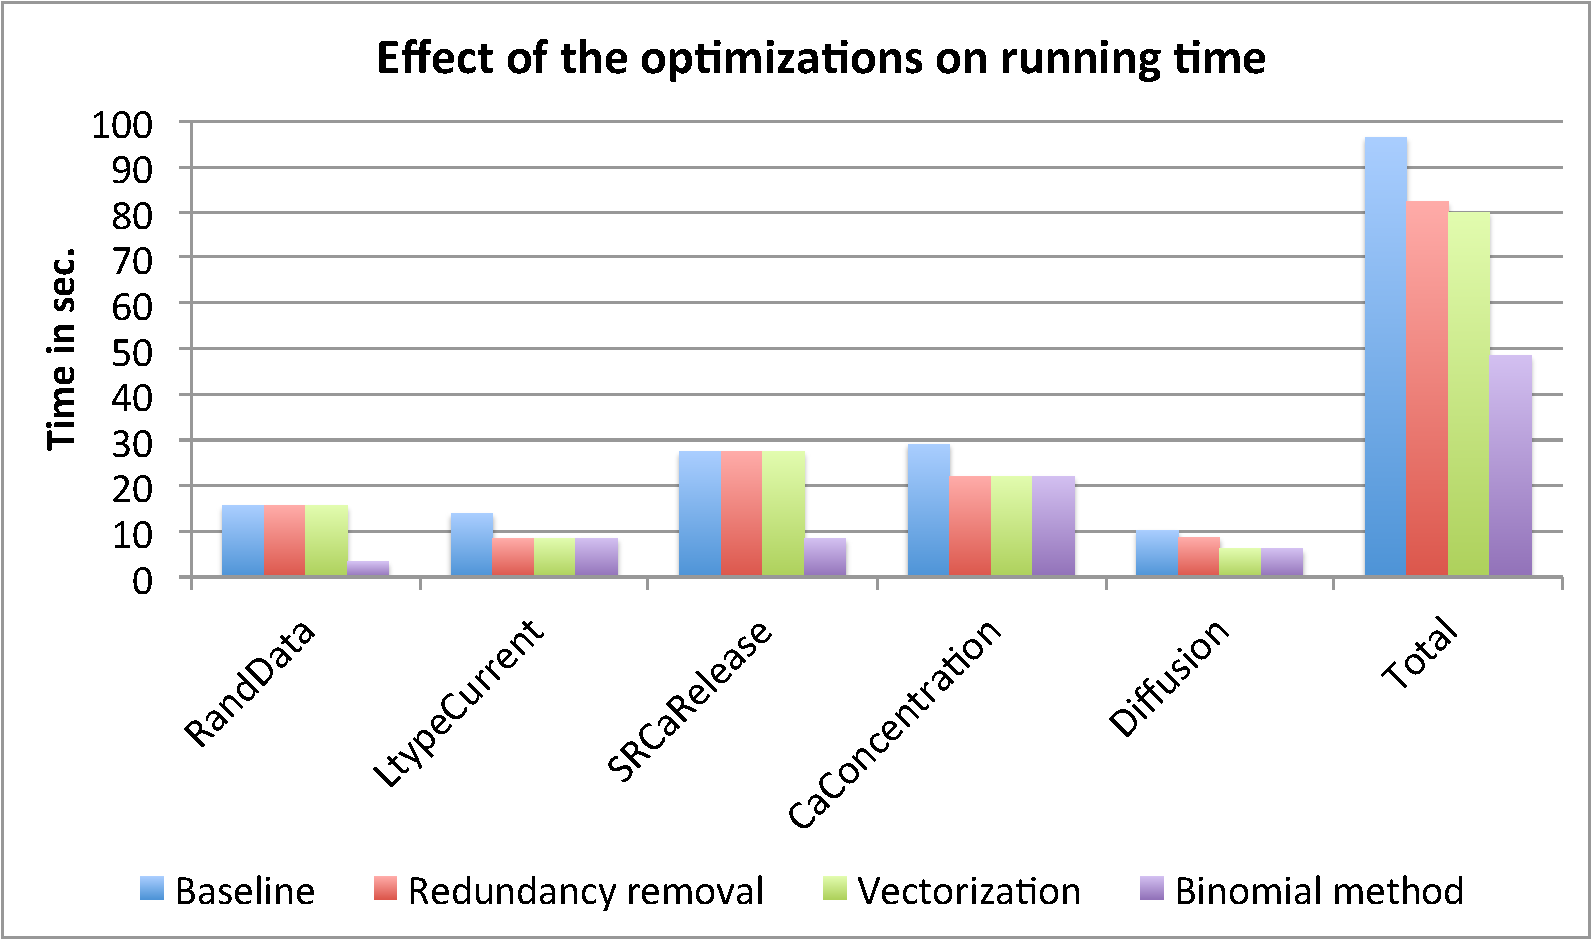
\includegraphics[width=\textwidth]{figs/optimization.pdf}
\caption{Performance improvement of the individual functions in {\tt computeCalciumInDyad} due to the different optimization techniques. The three optimizations are applied cumulatively. Thus, the values for the Binominal method reflect the sum of all improvements.}
\label{fig:optimizations}
\end{figure} 

\subsection{扩展性实验}
本章对弱扩展和强扩展都进行了试验,试验中模拟时长为$1000$ ms,对于两个扩展试验,分别都做了两个模拟试验,一个是细胞内的dyad数量设置为$100$个,另一个是细胞内dyad数量设置为$10000$。

在弱扩展试验中,本课题使用的计算节点的数目从$1$到$128$。当使用$100$个dyad时,为每个计算节点分配的心脏组织大小为$64\times64\times64$,$128$个计算节点上完成大小为$512\times256\times256$ 的心脏组织的模拟。对于$10000$个dyad来说,为每个计算节点分配的心脏组织大小为$16\times16\times16$,$128$个节点分配心脏组织大小为$128\times64\times64$。扩展性试验中,每秒钟能够完成的细胞计算量作为扩展性的衡量标准,一个细胞计算量是指一个时间步计算一个细胞。图\ref{scaling1}给出了弱扩展试验的结果,其中纵坐标代表细胞计算量,横坐标是使用的计算节点数。从结果看出,试验表现出很好的弱扩展性。

对于强扩展试验中细胞内dyad设置为$100$个时,心脏组织大小固定在$256\times256\times256$这个规模,而对于每个细胞内dyad数量为$10000$,心脏组织规模为$32\times32\times32$,由于存储的需求,强扩展试验中最少需要$8$ 个计算节点。与弱扩展试验中类似,仍然采用细胞计算量这个指标,图\ref{scaling1}也展示了强扩展试验的结果。强扩展基本上取得了与弱扩展一样的性能。性能上细微的差别可以通过通信量来解释,强扩展试验中通信量会比弱扩展试验大些,而在现有的实现中,通信暂且未做优化。

由于心脏细胞模拟是计算密集型的应用,因此,无论是在弱扩展,还是强扩展试验中,模拟试验都表现了很好的扩展性。通过每秒细胞计算量这个指标,可以对任何规模的心脏组织在给定计算资源的条件下需要模拟的时间进行预测。

\begin{figure}[htb]
\center
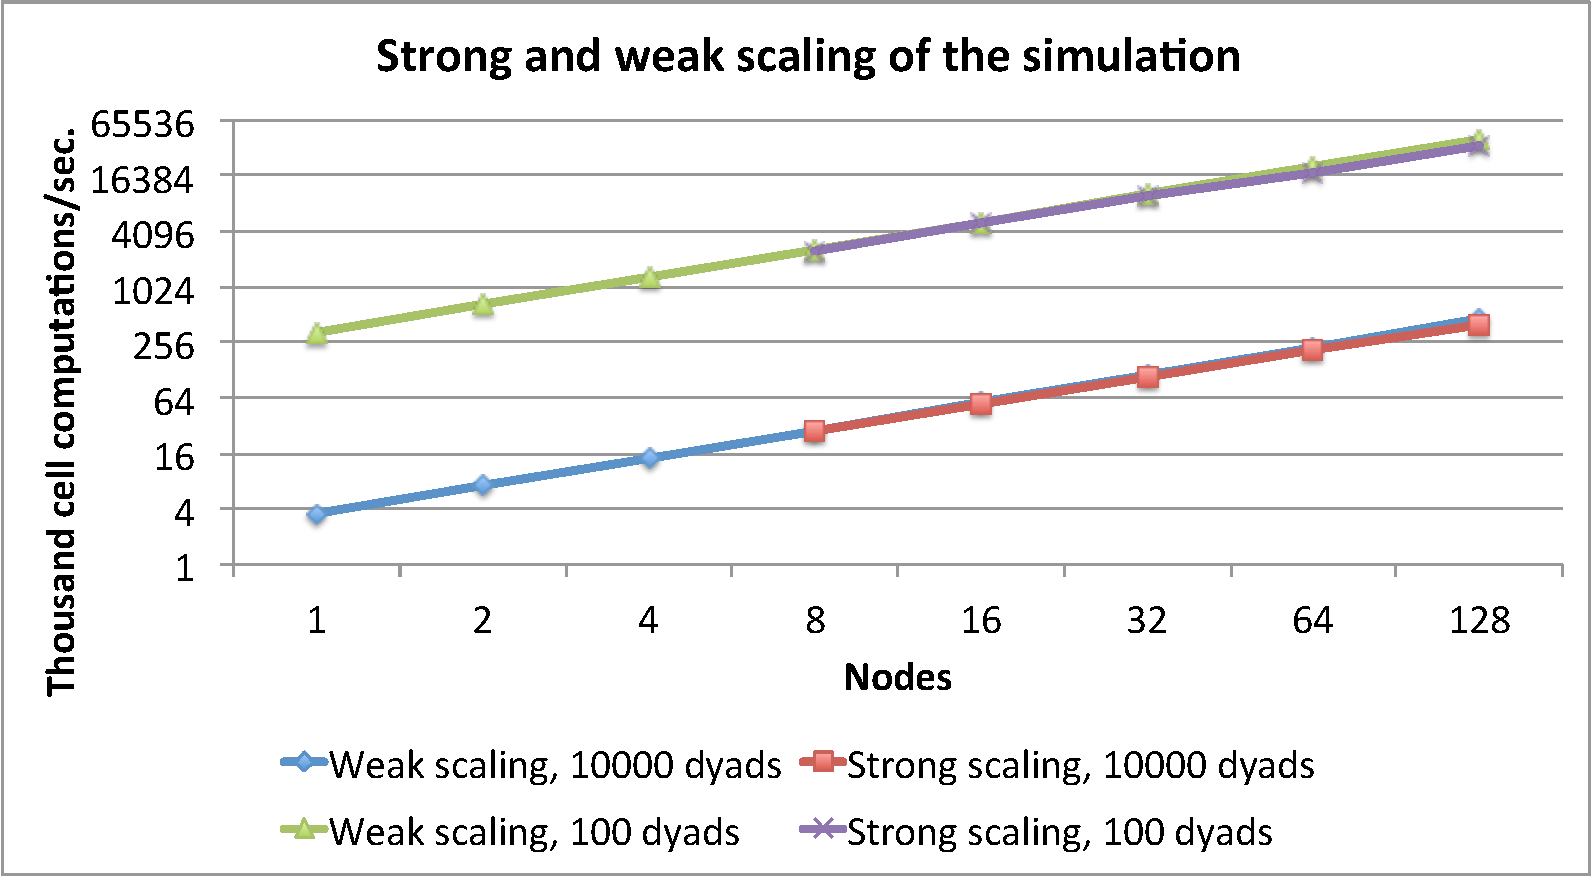
\includegraphics[width=\textwidth]{figs/scaling.pdf}
\caption{Performance of weak and strong scaling tests of tissue simulations. The $Y$ axis shows performance measured via the number of cell computations (i.e.~time steps for a single cell) performed for each wall-clock second of simulation time used. }
\label{scaling1}
\end{figure} 


\subsection{细胞内离子活动实验}

在图\ref{fig:calciumcell}中,我们展示了人类心脏细胞内正常的心跳过程中钙离子处理变化过程。试验以不同的尺度展示了心脏组织的中心细胞内钙离子处理结果。图\ref{fig:calciumcell}中A部分显示了在两次连续的心脏中活动电势的变化;图\ref{fig:calciumcell}中B部分是位于细胞中心的dyad内处于打开状态的RyR的数目,这些数目是按照\ref{binom}通过二项分布的方法计算出来的。模拟结果表明,在活动电势变化期间,大部分RyR是出于打开状态的,随着这些通道的打开,在dyad内的$Ca_{ds}$浓度迅速上升到$500\mu$M,以及$Ca_{ss}$上升到$0.1$mM,具体变换过程可以从图\ref{fig:calciumcell}中的C和D观察到。对于亚细胞层级,对细胞内的Ca ($Ca_{i}$)进行模拟的线扫描影像表明,细胞内所有dyad内的钙离子释放是同步发生的(参考图\ref{fig:calciumcell}的F)。整个细胞内相关的$Ca_i$为图\ref{fig:calciumcell}中G所示,以及H未整个细胞的JSR。总之,这些结果描述了正常心脏跳动过程中的不同尺度的钙离子处理过程,包括dyad级、亚细胞级以及细胞级。

\begin{figure}[htb]
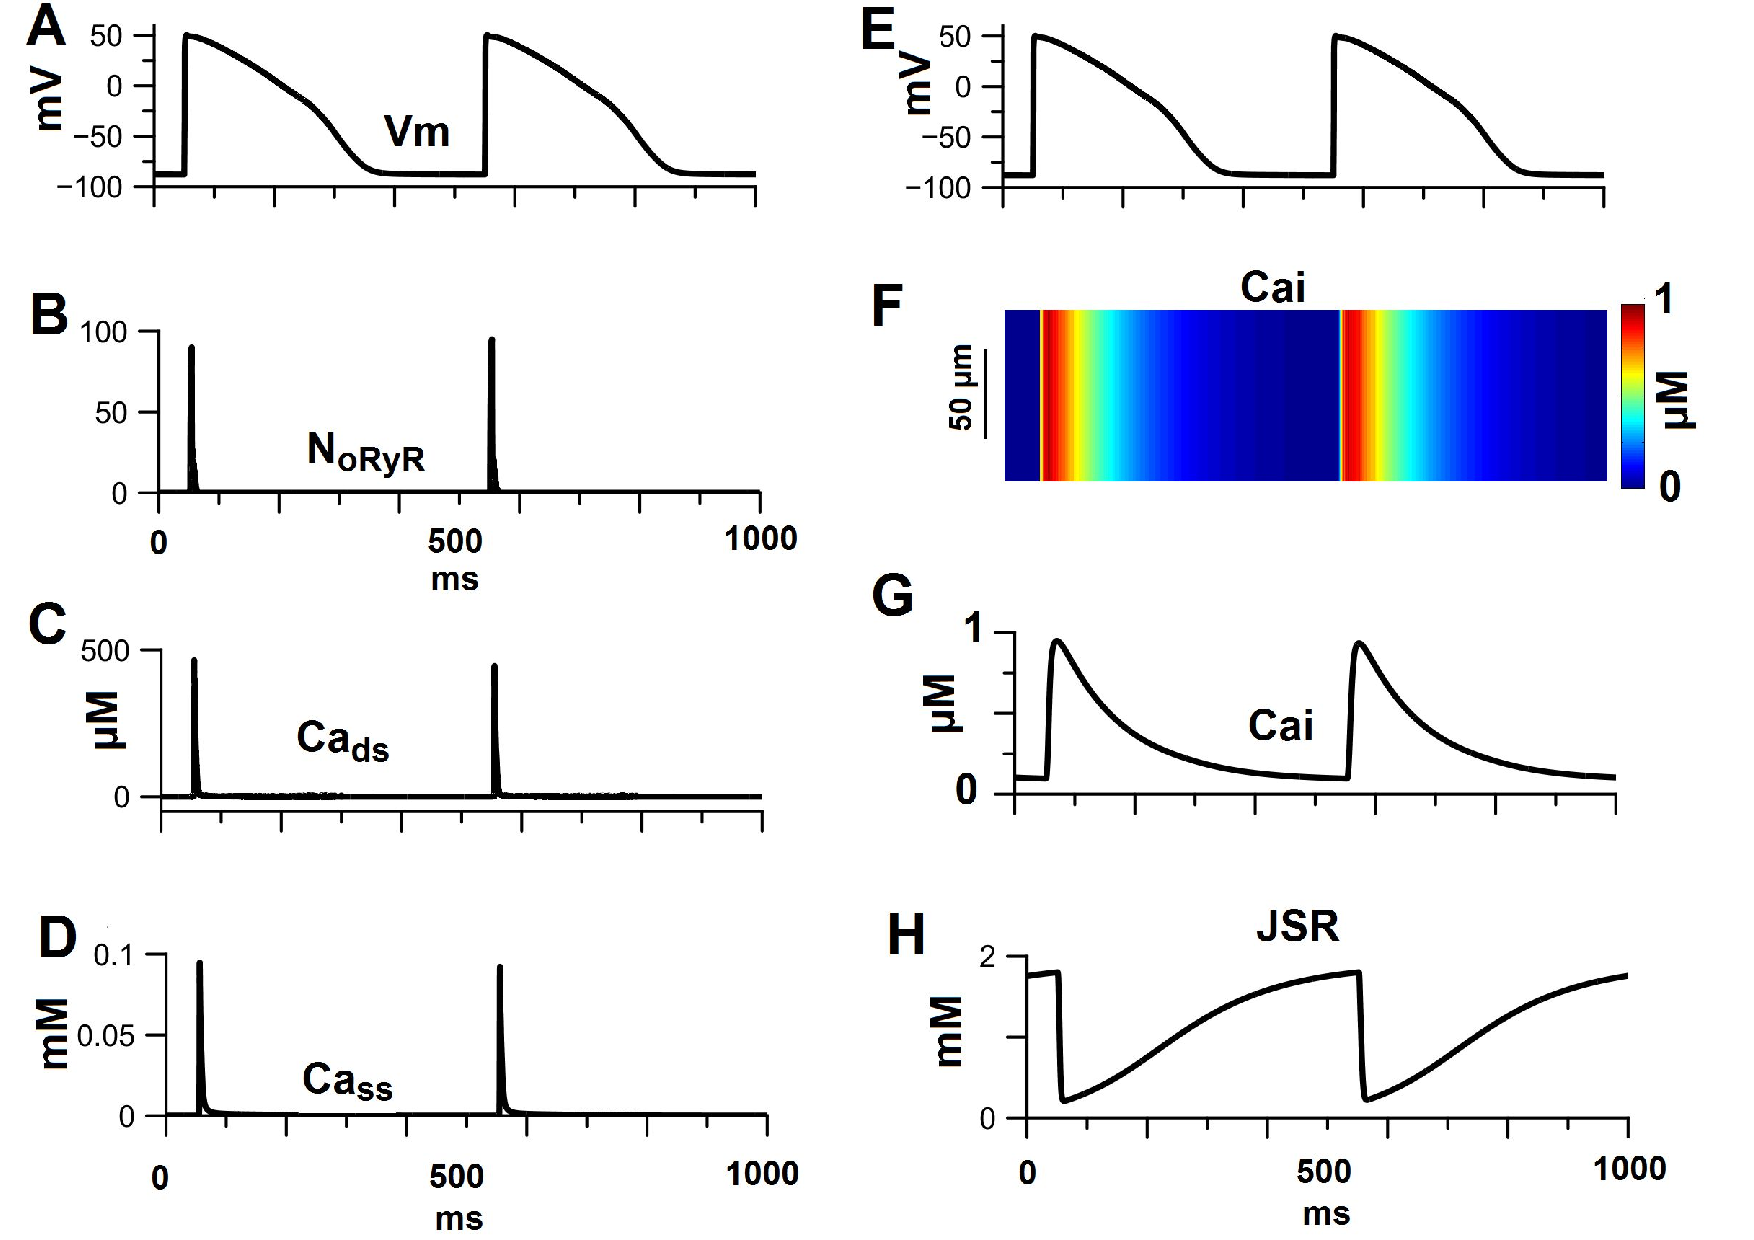
\includegraphics[width=\textwidth]{figs/calcium.pdf}
%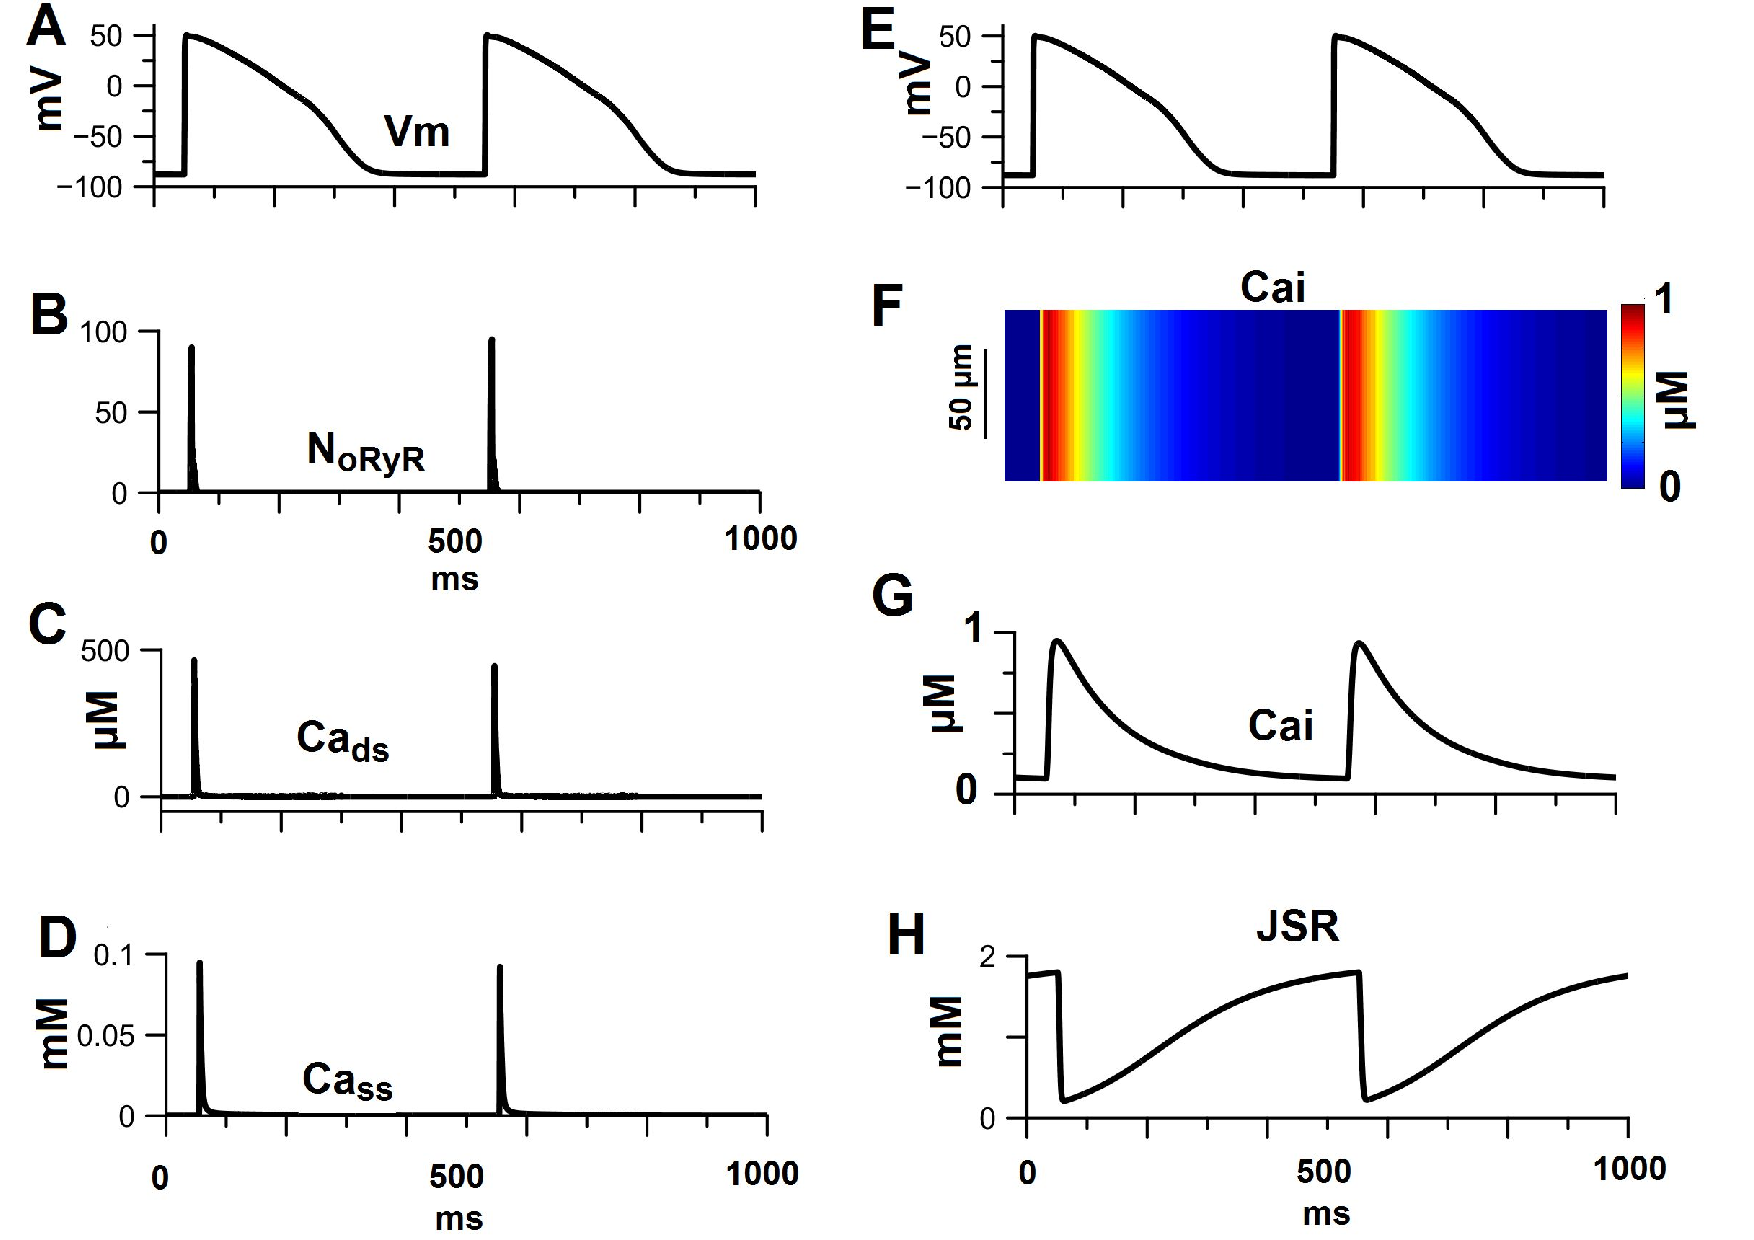
\includegraphics[scale=0.8]{figs/calcium.pdf}
\caption{Calcium handling in a cell in a human tissue during normal excitation. (A) Action Potential. (B) Number of open RyRs ($N_oRyR$) in the center dyad of the cell. (C) Dyadic space calcium ($Ca_{ds}$) (D) Submembrane space calcium ($Ca_{ss}$) (F) Simulated linescan image of intracellular Ca ($Ca_i$ (G) Whole-cell $Ca_i$ and (H) Whole-cell junctional sarcoplasmic reticulum (JSR). The 3D tissue was plane-stimulated at an edge at a cycle length(CL)=500 ms. Last two steady-state beats are shown.}
\label{fig:calciumcell}
\end{figure}

\subsection{心脏组织内异常活动模拟}

图\ref{arrhythmia}在3D心脏组织中的膜电位变化图,在时刻t = 0 ms,心脏组织的边缘受到一个刺激,经过一段时间的电压传播,在t = 600 ms时,心脏组织的一部分细胞受到新的刺激,在新刺激和之前的电压扩散的双重影响下,最后在心脏组织内部形成一个卷波。从心脏组织中的三个位置A、B、C的细胞进行采样,这三个位置的膜电位变化如图\ref{arrhythmia}中下半部分所示。在整个模拟过程中,卷波非常稳定,没有产生新的小波。这个模拟试验表明了本课题实现的这个组织模拟器能够模拟出在心脏组织的异常功能研究中非常有用的卷波。

\begin{figure}[htbp]
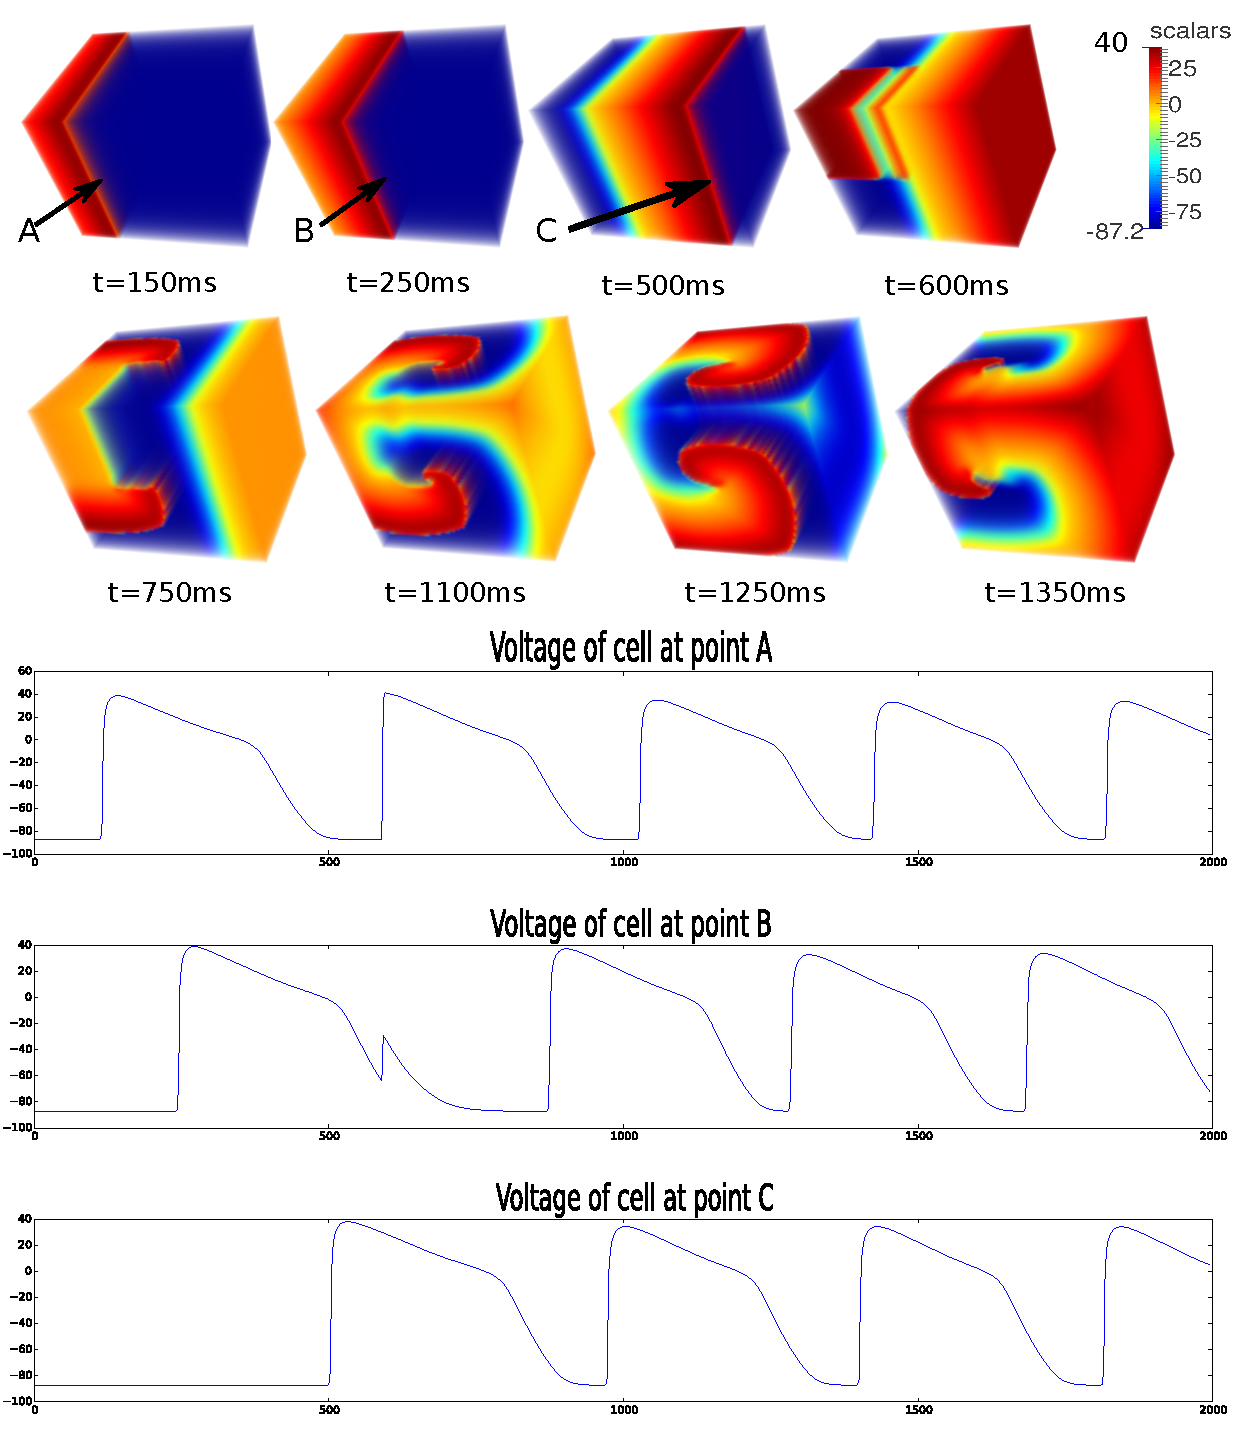
\includegraphics[width=\textwidth]{figs/voltage}
\caption{Simulation of scroll waves in a 3D tissue. The top part shows voltage snapshots at different time points. The bottom section shows membrane potentials at three different locations in the tissue.}
\label{arrhythmia}
\end{figure}

\section{小结}
本章介绍了3D组织模拟的精细模型,采用了细胞内多尺度钙离子处理模型对心脏组织细胞的电活动和钙离子处理过程进行模拟。以往针对3D心脏组织的许多研究都是利用全细胞钙离子处理模型,而多尺度的钙离子处理模型并没有在组织模拟中广泛使用,其中的原因一方面是因为多尺度模型模拟对计算需求巨大;另一方面是当今缺少针对这些计算的有效的数值方法和算法。而本课题提出了一个多尺度模拟的模型,并在大规模的集群系统实现了。在实现过程中,本课题采用了多种优化方法,首先是减少了心脏组织细胞的模型中的很多变量的重复计算,其次是根据硬件平台的并行计算资源对3D心脏组织进行了多级并行,最后对心脏组织模拟的核心模拟过程采用了二项分布的方法。这些优化方法使得模拟的时间减少了一半。对性能提升效果最明显的是二项分布方法的引入,二项分布方法减少了对随机数的使用,可以节省大量用于产生随机数的时间。

弱扩展测试针对不同的组织规模,在不同数目的计算节点上基本保持了相同的计算时间。而强扩展试验中,随着计算节点数目的增加,计算时间基本保持了一个线性下降的关系。这些结果表明了将更大规模的心脏组织模拟映射到更大规模的集群系统中进行模拟成为可能。最后通过试验证明了本课题研究针对心脏组织细胞内的钙离子处理模拟与已经发表的工作\upcite{o2011simulation}的结论是一致的。试验也证明了本课题研究的模型能够模拟3D心脏组织的心率失常等问题。

总结本章工作,本章提出了一个精细的3D心脏组织模拟模型,这个模型能够模拟人类心脏组织细胞内的电活动和钙离子处理过程,通过采用多个优化方法,最后将模型在大规模多核系统高效地实现了。试验中的扩展性结果表明全心脏的模拟在当前最快的超级计算上进行模拟也是可能的。在下一章中,本课题将进一步提高3D组织模拟器的性能,并且将已有的实现移植到更快的硬件加速器系统中。这将逐渐从多个尺度增加研究人员对心脏病理的机制的理解。





\chapter{心脏组织模拟在天河2异构系统上的并行优化}
\label{icpads}

\section{引言}
在\ref{ICA3PP}中,已经介绍了心脏组织模拟在研究心律失常等各种心脏疾病具有重要的作用,心脏组织模拟的模型越详细,对计算的需求越大,在\ref{ICA3PP}中也已经介绍了本课题在多核CPU的集群系统上做的一些工作,采用了MPI+OpenMP的并行编程方法,对一定规模的心脏组织进行了模拟。但如果想对更大规模的心脏组织模拟则需要计算能力更强的处理器或者加速器构成的超大规模集群系统。文献中\upcite{GPUcell}采用了GPU在细胞层级对模拟进行加速,利用加速器对模拟进行加速不失为一种好的选择。

基于现有的计算资源,本课题将心脏组织模拟移植到超级异构集群系统即天河2号超级计算机\upcite{tianhe}上。天河2号超级计算机系统在TOP500排名中位居第二,它的每个计算节点都是由Intel CPU与Intel PHI协处理器构成的异构系统。

众核加速器的每个芯片集成了大量的简单小核,非常适合作为高性能计算系统的核心计算部件。Intel的Xeon Phi协处理器和GPU是两种典型的众核加速器。本课题将面向天河2号超级计算机系统实现心脏组织的3D模拟,天河2号超级计算机系统采用多核CPU作为控制核心以及Intel Xeon Phi协处理器作为加速部件。天河2号系统的峰值性能可以达到54.9PFlops,实测性能可以达到33.86PFlops。

天河2号系统具有很强的计算能力,但天河2号作为复杂的异构系统,这给天河2号上的并行编程带来了诸多挑战。因此,对于一个应用能否在天河2号上取得很好的性能,取决于并行实现。对于天河2号系统来说,除了需要高效地充分利用其大量的硬件线程,单个物理线程上的SIMD向量化也需要尽可能地得到发挥。物理线程的并行可以通过OpenMP编程实现,或者通过一个MPI进程内创建多个OpenMP线程控制多个物理线程,SIMD向量化理论上能够将双精度的浮点性能提升8倍,SIMD向量化可以在代码中添加编译指导语句,借助编译器对代码自动向量化,或者采用AVX-512向量指令\upcite{XEONPHI}手动对代码进行向量化。编译器自动向量化的方法只针对代码中比较规则的计算,而对于不规则的代码则需要通过手动向量化实现SIMD。

对于由CPU和Xeon Phi构成的异构系统来说,多核CPU的性能同样不容忽略,目前每个计算节点内CPU核的个数一般在8到18之间,然而每个CPU核使用更高的时钟频率,功能也更加强大,更加灵活,适合做一些控制的任务。对于一些特殊的计算,比如很难实现SIMD或者是存储带宽受限,则多核CPU上的实现性能可以达到协处理器上的实现性能。因此异构节点上CPU核与Xeon Phi协处理器应该协同起来,充分发挥异构系统的性能。然而,从编程的角度来说,异构计算可能带来新的问题,比如,对于SIMD向量化,CPU采用不同的AVX指令集,因为CPU的SIMD指令是针对256位的向量计算。异构计算还可能需要解决优化CPU和Xeon Phi间的数据传输问题以及CPU和Xeon Phi间的负载均衡问题等。

本课题的目标是将心脏组织的模拟移植到天河2号的超级异构计算机系统中,为了有效地使用天河2号的硬件资源,需要将模拟的计算过程进行多层次的并行开发,包括计算节点间的并行、节点内CPU和Phi设备间的并行、Phi设备上众核间的并行以及Phi设备的每个计算核心内SIMD的并行。这无疑会给编程带来巨大的挑战,这正是本课题需要解决的问题。

本章内容安排如下,首先将介绍天河2号超级计算机系统的硬件结构;然后将介绍心脏组织模拟在天河2号系统上的高性能并行实现与优化,主要利用硬件结构的特点,将心脏组织模拟的并行映射到具体的硬件中执行,并对其中的关键计算部分进行优化;最后是对试验结果评测,主要测试了心脏组织模拟在天河2号上单节点内的Phi设备上的性能、单节点的性能以及多节点的性能。试验结果表明,本课题针对天河2号异构集群系统开发出了一个高效的心脏组织模拟器。

\section{目标硬件体系结构}

天河2号超级计算系统包含16000个计算节点,每个计算节点有3个Intel Xeon Phi协处理器和2个Intel Xeon E5-2692v2 Ivy Bridge CPU处理器。因此,天河2号系统共有48000个Xeon Phi以及3200个Intel Xeon CPU。Xeon Phi的模型为31S1P(即Knigths Corner体系结构),每个Xeon Phi有57个核心,频率为1.1GHz,每个CPU有12和核心,频率为2.2GHz。

Intel Xeon Phi协处理器是一个基于众核设计的硬件加速器,与传统的多核CPU不同的是,Phi协处理器是由大量的性能相对较弱的小核构成的,这些小核以环形的结构相连,每个小核支持512位宽的向量处理,具有64KB大小的L1 cache以及512KB大小的L2 cache,所有小核的cache支持一致性协议。Xeon Phi的这种设计使得它不适合处理串行程序,但非常适合处理并行程度高的程序。对于Xeon CPU来说,CPU中的每个小核具有64KB大小的L1 cache,256KB大小的L2 cache,并且Xeon CPU具有被12个小核共享的30MB大小的L3 cache。

Xeon Phi的理论峰值双精度性能可以根据参数理论上计算出来,它的向量位宽为512位,所以每次可以处理8个双进度浮点运算或者16个单精度浮点运算,根据前面介绍的频率和小核的个数,可以计算出一个Xeon Phi的单精度浮点峰值性能可以达到$1001$ GFlop/s。然而,在实际中,一般不能取得这么高的性能,CPU的计算性能也不容忽略,峰值性能可以达到$211$ GFlop/s,实际中应该充分发挥Xeon CPU和Xeon Phi两种计算资源的性能。

对于节点间的通信问题,天河2号系统采用了自己定制的名为TH Express-2的互联系统,这是一个胖树的拓扑结构。理论上说,Xeon Phi上是支持MPI通信的,单节点内Xeon Phi间采用MPI通信对性能不会有太大损失,但对于处于不同节点的Xeon Phi间的通信,采用MPI通信并不是很高效的方法。因此,本课题采用的策略是一个节点由一个MPI进程控制,然后在MPI进程内为每一个Xeon Phi创建一个线程,每个线程负责管理一个Xeon Phi,Xeon CPU和Xeon Phi间的通信采用Intel的SCIF/COI接口\upcite{SCIFCOI}进行通信。由于SCIF/COI接口较底层,编程会相对较复杂,但会取得很好的性能。

Xeon Phi的57个小核中,有一个小核是保留给操作系统使用的,因此,真正能用于计算的小核个数只有56个。每个小核能同时运行4个物理线程,但对于给定的一个线程,它不会在连续的两个时钟周期都运行,意味一个Xeon Phi内只有有效的112个线程能以$1.1$ GHz的时钟周期运行。当运行224个线程时,每个线程是以系统的时钟周期的一半运行的。Xeon Phi协处理器的DDR5设备存储大小为8GB,小核访问设备全局存储的峰值带宽\upcite{xeon_phi_peak}为$320$ GB/s。然而,即使在理想情况下,对于很多应用来说,峰值带宽的一半还是可以达到的\upcite{testdrivingPhi}。


\section{心脏组织模拟的高性能并行实现与优化}

。。。。。。。。

\subsection{心脏组织模拟的tissue-级并行}
心脏组织模拟的全部计算任务具有多个层次的并行性,结合目标体系结构的特点,本课题对心脏组织模拟的计算任务进行分解,分解成多个层次。在最顶层分解中,心脏组织细胞以3D网格的方式结合在一起。每一个计算节点被分配到一定数量的细胞进行处理,这些细胞构成一个子域,子域的形状也是一个立方体。处于子域边界的细胞,它们的电压值在进行扩撒计算前需要与相邻的子域边界的细胞的电压值交换。细胞的电压值交换是通过CPU间的MPI通信实现的,采用了标准的halo交换方法。

对于每个子域在节点内的CPU和Phis间的细胞划分,本课题没有对立方体构成的子域进行规则的划分,因为这会导致CPU与Phis间负载的不均衡,而是根据CPU和Phi的计算能力分配相应比例的细胞给CPU和Phi这两种计算设备。这种策略需要对CPU和Phis处理的所有的细胞的电压值进行交换,CPU和Phi间的通信采用Intel的SCIF/COI通信接口实现。虽然这种方法会增加节点内CPU和Phi间的通信,但付出的代价会比因为负载不均问题产生的额外开销小。图\ref{nodeload}是节点内对子域构成的立方体细胞划分的示意图,不同颜色的部分代表分配给不同的计算设备。

 \begin{figure}[bth]
\center
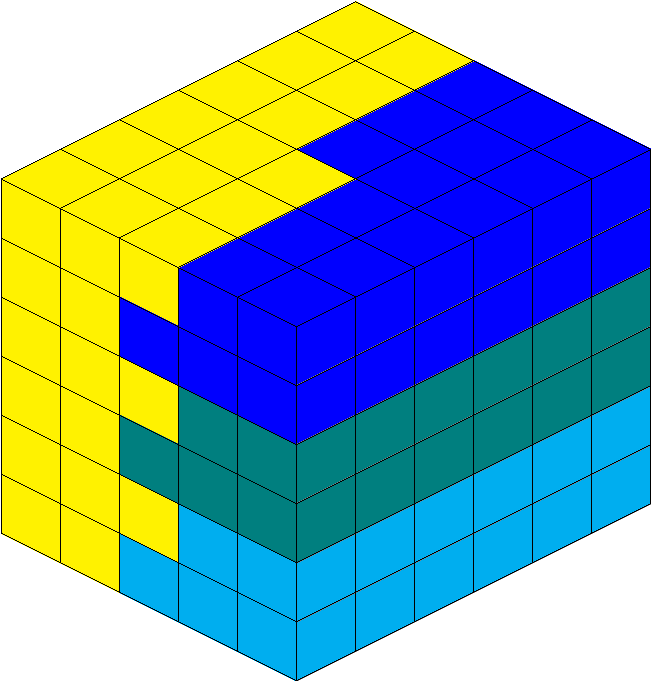
\includegraphics[scale=0.5]{figs/cube}
\caption{Example of the intra-node decomposition of a subdomain. Cells allocated to the Phis are shown in \textcolor{blue}{blue}, \color{teal}{teal}, \textcolor{black}{and} \textcolor{cyan}{cyan}, \textcolor{black}{while the CPU cells are shown in} \textcolor{yellow}{yellow}.}
\label{nodeload}
\end{figure}

In addition, the limited memory ($8$ GB) and the large number of concurrent threads ($224$) of the Xeon Phi mandate further constraints. Due to the large number of dyads, each cell 
requires approximately $3$MB of memory, which limits the number of cells on each Phi to about $2500$. This in turn implies that each thread computes only a small number of cells (up to $12$) per time step, which makes the computation quite sensitive to unbalanced loads. Therefore, each Phi should be assigned a number of cells which is a multiple of $224$ for 
optimum load balance within the device. 


During preliminary experiments, we found that the relative computational speed between the host CPU (two sockets) and one Phi is about $1.5 : 1$. Together with the above restrictions, we found the optimal subdomain size to be $20\times20\times20$, with $8\times224=1792$ cells assigned to each Phi and the remaining $8000-3\times1792=2624$ cells assigned to the host CPU, which thus processes $32.8\%$ of the cells. Even though we do not always use them in our experiments, proportionally smaller or larger subdomains obeying the same ratios are also possible. Furthermore, we note that performance may vary slightly between the computations, which makes it impossible to have a strictly optimal load balance. 
 
\subsection{心脏组织模拟的cell-级并行}

\subsection{心脏组织模拟的dyad-级并行}

\subsection{心脏组织模拟中随机数生成}


\subsection{代码优化}



\section{实验结果与分析}
\subsection{实验设置}

\subsubsection{心脏组织模拟单设备性能}

\subsection{心脏组织模拟的单节点性能}

\subsection{心脏组织模拟的多节点性能}

\subsection{心脏组织模拟试验}

\section{小结}
